% Tutamen: A Second-Generation Secret Storage as a Service Platform
% Paper
%
% 2016
%
% Andy Sayler
% Taylor Andrews
% Matt Monaco
% Dirk Grunwald


\documentclass[letterpaper,twocolumn,10pt]{article}

% System Packages
\usepackage{epsfig}
\usepackage{float}
\usepackage{caption}
\usepackage{subcaption}
\usepackage{tabu}
\usepackage{color}
\usepackage{hyperref}
\usepackage{url}
\usepackage{listings}
\usepackage{authblk}

% Local Packages
\usepackage{usenix}

% Package Options
\hypersetup{
    colorlinks,
    citecolor=black,
    filecolor=black,
    linkcolor=black,
    urlcolor=black
}
\lstset{
  language={},
  basicstyle=\footnotesize,
  numbers=left,
  numberstyle=\tiny,
  stepnumber=1,
  numbersep=5pt,
  showspaces=false,
  showstringspaces=false,
  showtabs=false,
  tabsize=4,
  captionpos=b,
  breaklines=true,
  breakatwhitespace=false,
  frame=single,
  frameround=tttt
}
\lstdefinelanguage{JavaScript}{
  keywords={break, case, catch, continue, debugger, default, delete,
    do, else, finally, for, function, if, in, instanceof, new, return,
    switch, this, throw, try, typeof, var, void, while, with, true,
    false, null},
  morecomment=[l]{//},
  morecomment=[s]{/*}{*/},
  morestring=[b]',
  morestring=[b]'',
  sensitive=true
}

% Macros
\newenvironment{packed_enum}{
\begin{enumerate}
  \setlength{\itemsep}{1pt}
  \setlength{\parskip}{0pt}
  \setlength{\parsep}{0pt}
}{\end{enumerate}}

\newenvironment{packed_item}{
\begin{itemize}
  \setlength{\itemsep}{1pt}
  \setlength{\parskip}{0pt}
  \setlength{\parsep}{0pt}
}{\end{itemize}}

\newenvironment{packed_desc}{
\begin{description}
  \setlength{\itemsep}{1pt}
  \setlength{\parskip}{0pt}
  \setlength{\parsep}{0pt}
}{\end{description}}


% Other Options
\clubpenalty = 10000
\widowpenalty = 10000

% Start
\begin{document}

%don't want date printed
\date{}

%make title bold and 14 pt font (Latex default is non-bold, 16 pt)
\title{\Large \bf Tutamen: A Next Generation Secret Storage Platform}

% start author
\author{Andy Sayler}
\author{Taylor Andrews}
\author{Matt Monaco}
\author{Dirk Grunwald}
\affil{University of Colorado}
% end author

\maketitle

% Use the following at camera-ready time to suppress page numbers.
% Comment it out when you first submit the paper for review.
%\thispagestyle{empty}

\subsection*{Abstract}

The storage and management of secrets (encryption keys, passwords,
etc) are significant opens problems in the modern age of cloud-based,
ephemeral computing infrastructure. How do we store and control access
to the secrets necessary to configure and operate a range of modern
technologies without sacrificing security and privacy requirements or
significantly curtailing the desirable capabilities of our
applications? As an answer to this question, we propose Tutamen - a
next generation secret-storage service. Tutamen offers a number of
desirable secret storage properties not present in existing secret
storage solutions, including the ability to shard secrets across
multiple storage providers - ensuring both redundancy and security,
the ability to share secrets between users, and the ability to require
contextual and out-of-band authentication parameters as a prerequisite
to gaining secret access. These properties have allowed us to leverage
Tutamen support a variety of use cases not easily realizable using
existing systems such as providing autonomous full-disk encryption to
headless servers and providing client-side encryption for files stored
atop cloud-based file lockers or networked file systems while also
supporting sharing and multi-device access to such files. In this
paper, we present the nature of the secret storage problem, Tutamen's
design and architecture, the implementation of our Tutamen prototype,
and several of the applications in which we have implemented
Tutamen-based secret storage to achieve previously unattainable goals
whiles till meeting a variety of security and privacy requirements.

\section{Introduction}
\label{sec:intro}

How best to store and manage secrets -- the bits of tightly controlled
data necessary to ensure or bootstrap the security of computing
systems and services -- has always been a non-trivial problem. As we
continue to move toward computing and storage platforms controlled by
third parties, and embrace modern trends toward ephemeral
infrastructure, the secret storage problem only becomes more prevalent
and critical to solve.

Tutamen\footnote{Latin -- A means of protection or defense.} is our
attempt to solve the secret storage problem in a manner that allows
the user to adhere to a range of security and privacy requirements
without sacrificing functionality in the process. Tutamen is a next
generation secret storage platform. It builds on our previous secret
storage efforts~\cite{custos-trios} and strives to offer features not
provided by the various secret storage systems available today. In
this paper, we offer several contributions:

\begin{packed_item}
\item The design, implementation, and evaluation of a secret storage
  system with support for several novel features including:
  \begin{packed_item}
  \item Modular authentication modules designed to add use-case
    flexibility through the use of contextual, multi-factor, and
    alternate-band (e.g. SMS text messages) authentication mechanisms.
  \item The ability to operate atop minimally trusted infrastructure
    by leveraging multiple storage and access control providers to
    achieve both redundancy and to mitigate trust.
  \end{packed_item}
\item Several practical demonstrations of how a secret storage system
  with such features can be integrated with real-world applications to
  offer desirable features in a secure and easy-to-use manner.
\end{packed_item}

\subsection{The Need for Secret Storage}

Computing systems today invade every contour of our lives -- from the
fitness trackers on our wrists, to our ``smart'' home appliances, to
the server infrastructure required to support the range of web sites
and services we interact with every day. With this explosion of
computing systems has come an equally large explosion in the amount of
data stored by and about us. While some of this data is designed to be
public (i.e. the entries on Wikipedia), much of it is not, requiring
the enforcement of various privacy and security guarantees with
respect to its handling and storage. The basis of providing such
guarantees relies on our ability to store and selectively share
secrets ranging from the keys used to encrypt our data to the
passwords used to protect our online accounts. How best to store and
manage these secrets is thus a critical question -- the answer to
which forms the foundation to all of computing's higher level security
and privacy guarantees.

Beyond the need to bootstrap a variety of security guarantees, there
are several other factors driving the need for robust secrete storage
solutions. On the system administration front, the trend toward
ephemeral infrastructure cable of rapidly scaling up or down is
driving the adoption of configuration management systems such as
puppet~\cite{puppet} or chef~\cite{chef}. Such systems, however, do
not tend to have suitable mechanisms for enforcing the security and
privacy requirements inherent to storing secrets. Despite this,
configuration data often contains a variety of secrets such as SSH
keys, TLS/SSL keys, file encryption keys, and the tokens or
credentials necessary to authenticate to external APIs and services.

Similarly, on the end-user front, the need for suitable secret storage
systems is being driven by a rapid expansion of the number of sites
and services to which users must authenticate themselves, as well as
by the growing expanse of digital data users wish to protect. Indeed,
the popularity of password management systems such as
LastPass~\cite{lastpass} or 1Password~\cite{onepassword} as well as
user demands for encryption support on their
devices~\cite{intercept-cookencryption} demonstrate the importance of
secret storage, and the applications it enables, to end users.

\subsection{The Ideal Secret Storage System}

Unlike standard configuration management systems, or even specific
secret storage systems such as password managers, a general purpose
secret storage presents a number of unique requirements including the
following capabilities:

\begin{packed_item}
\item Store a wide-range of arbitrary secret data
\item Store secret data in a secure manner
\item Enforce fine-grained access control requirements
\item Support a range of authentication sources/methods
\item Provide audit logs tracking secret access history
\end{packed_item}

In response to these needs, a number of general purpose secret-storage
systems have been recently developed by industry, including
HashiCorp's Vault~\cite{vault}, Lyft's Confidant~\cite{confidant}, and
Square's Keywhiz~\cite{keywhiz}. These systems exist to fulfill some
or all of the requirements listed above. We believe, however, that
such systems are hindered by several key limitations. First, they
generally require at least one fully trusted server as the basis of
their security model, making them unsuitable for operation atop
untrusted infrastructure. Second, they tend to lack support for use
cases requiring autonomous or remote access to secret material in a
secure manner. These deficiencies give rise to a few more secret
storage requirements:

\begin{packed_item}
\item Avoidance of the need to place a high degree of trust in any
  single system outside the application that wishes to store a secret.
\item Ability to support a range of secret access use-cases, including
  use cases where automatic or remote access to secrets is required.
\end{packed_item}

It is toward these final two requirements that Tutamen attempts to
advance the state of the art over existing secret storage systems. In
particular, Tutamen supports operational modes where no single entity
other than the application must be trusted. This allows users to
leverage third party secret storage providers running Tutamen servers
without having to place high degrees of trust in any single
provider. Tutamen also provides support for a modular authentication
interface. This interface makes Tutamen suitable for use in situations
where it is desirable to leverage external environmental information
to automatically evaluate the authenticity of a secret request are
where it is necessary to keep a human in the authentication loop
without actually requiring that the human be physically present or
connected to the application requesting a secret. For example, Tutamen
can be used to store the disk encryption keys required to boot a
headless server, and only release these keys to the server requesting
them when a human responds to a text message confirming the boot
request.

%%  LocalWords:  Tutamen LastPass HashiCorp's Lyft's Keywhiz OOB SMS

\section{The Tutamen Platform}
\label{sec:tutamen}

\subsection{Architecture}

The Tutamen Secret Storage platform has three main components:

\begin{packed_desc}
\item[Access Control Servers (ACS):] The systems responsible for
  storing and enforcing secret access control requirements and for
  authenticating clients making requests.
\item[Storage Servers (SS):] The systems responsible for storing
  secrets (or parts of secrets).
\item[Tutamen Applications (TA):] The systems leveraging the Tutamen
  platform to store and retrieve secrets.
\end{packed_desc}

In general, Tutamen communication occurs between applications and both
types of servers. Tutamen servers do not generally communicates with
each other directly -- with the one exception of storage servers
needing to download the public signing keys from each of the access
control servers with which they interact. All communication in Tutamen
takes place via HTTPS connections - and in some cases leverage mutual
TLS to require both client and server authentication.

Both access control and storage servers are designed to be used
individually or in sets. E.g. An applications may store their secret
on a single storage server and delegate access control to a single
access control server, or the applications may shard its secret across
multiple storage servers and delegate access control to multiple
access control servers, or any combination thereof. By separating the
access control duties from the secret storage duties, Tutamen offers
the end-user a high degree of flexibility to implement a range of
redundancy and trust requirements.

\subsubsection{Access Control Servers}

The Tutamen Access Control Servers are responsible with authenticating
Tutamen requests as well as storing and enforcing all access control
requirements. Access Control servers expose a number of core data
structures that reflect that manner in which they
operate. Figure~\ref{fig:tutamen:acstructs} shows these structures.

\begin{figure}[th]
  \centering
  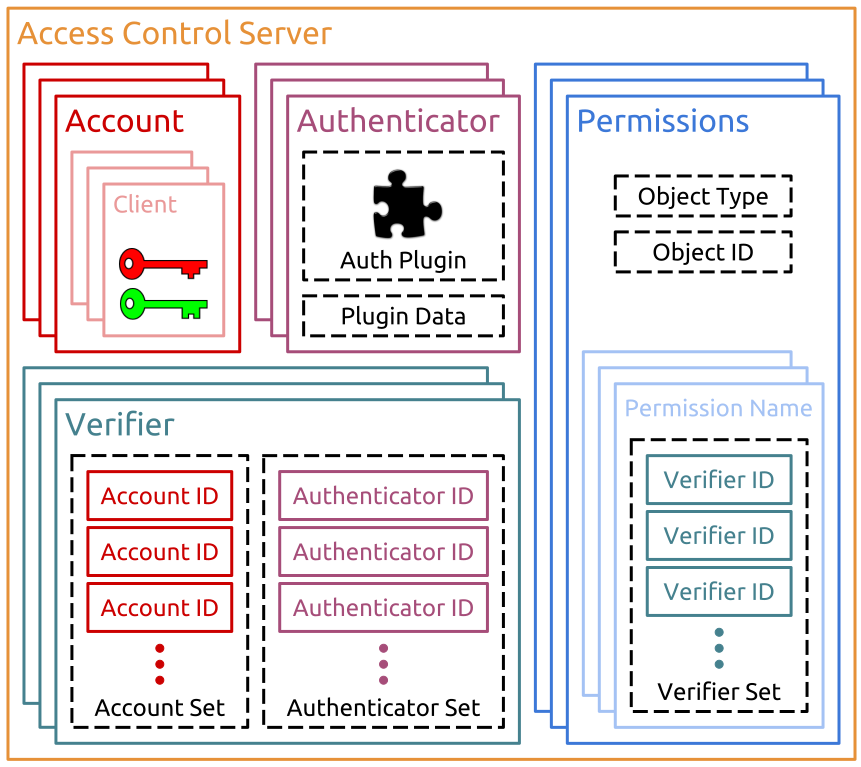
\includegraphics[width=\columnwidth]{./figs/pdf/tutamen-datastructures-ac.pdf}
  \caption{Access Control Server Data Structures}
  \label{fig:tutamen:acstructs}
\end{figure}

In order to track and control access from specific users - the ACS
uses per-user accounts. These accounts are generally designed to to
mapped to individual end-user, but they can be used to track any
singular entity to which one wishes to assign specific access control
privileges. Accounts thus form the basis of controlling and sharing
access to secretes via Tutamen. Within each account are one or more
clients. While accounts map to logically singular access control
entities, clients map to specific devices that will need to make
Tutamen requests. Each account has one or more clients. For example,
Jane Coworker would have a single account with one client for her
laptop, one for her desktop, and one for her phone.

Each client is associated with a single TLS key-pair used to
authenticate the client to the access control server. The access
control server doubles as the Certificate Authority administering
these certificates. When a new client is created it generates a local
RSA key and uses this key to generate an X509 Certificate Signing
Request~\cite{rfc5280}. This request is then sent to the access
control server where it awaits approval from an existing client in the
account. If approved, the CSR is used to generate a signed certificate
that is sent back to the new client for use in future access control
server communication. To facilitate bootstrapping new account, clients
keys and CSRs are also generated and sent with each new account
request. These are atomically approved and associated with the new
account -- i.e. the initial client is created in tandem with a new
account -- all subsequent clients are then approved by previously
approved clients.

While accounts and clients are used to identify specific
users/entities -- the Tutamen access control server also has
authenticators. Authenticators are modular mechanism used to implement
access control requirements beyond granting access on the basis of
accounts. For example, authenticators can support plugins to perform
additional contextual authentication requirements such as only
allowing access during specific times of day, or from requests
originating form specific IP addresses. Authenticators can also be
used to implement out-of-band authenticators mechanism such as
requesting approval for a specific request from a user via text
message or otherwise interfacing with eternal services to gain
approval.

Accounts and authenticators are combined via verifiers. A verifier
consist of a set of Accounts and a set of Authenticators. In order to
satisfy a verifier a request must originate form ONE of the Accounts
and must satisfy ALL of the authenticators plugins listed in the
verifier. A verifier may contain no Authenticators, in which case
authorization is granted solely on the basis of accounts.

The final component of the Tutamen access control specification are
permission groups. Each permission group corresponds to a specific
object (identified via the combination of an object type and an object
ID) within the Tutamen ecosystem. A permission groups contains one or
more permissions - each corresponding to a specific class of actions
that can be preformed on the corresponding object. Each permission
contains a set of verifiers. In order to be granted a given permission
a request must satisfy at least one of the verifiers in this set.

\subsection{Security and Trust}

\subsection{Implementation}

%%  LocalWords:  Tutamen ACS HTTPS CSR CSRs Authenticators verifiers
%%  LocalWords:  authenticators


\section{Applications}
\label{sec:apps}

\subsection{Full Disk Encryption}

\subsection{VM Image Encryption}

\subsection{Encrypted File Locker}

\section{Evaluation}
\label{sec:eval}

\subsection{Usage}

\subsection{Discussion}

\section{Conclusion}
\label{sec:conclusion}

\subsection{Future Work}

% DoS of UUIDs
% Audting Logging

{
  \footnotesize
  \bibliographystyle{acm}
  \bibliography{refs}
}

\end{document}

%%  LocalWords:  Tutamen Tutamen's OOB
